\documentclass[10pt,a4paper]{report}
\usepackage[utf8]{inputenc}
\usepackage[portuguese]{babel}
\usepackage[T1]{fontenc}
\usepackage{amsmath}
\usepackage{amsfonts}
\usepackage{amssymb}
\usepackage{graphicx}

\usepackage{titlesec}
\usepackage{termcal}
\usepackage{hyperref}

\graphicspath{{./img/}}

\author{Lucas Lopes Costa}
\title{Relatório}

\titleformat{\chapter}{\normalfont\huge}{\thechapter.}{20pt}{\huge\bf}

\setcounter{tocdepth}{3}

\begin{document}
\begin{titlepage}
	\centering
	%\includegraphics[width=0.15\textwidth]{example-image-1x1}\par\vspace{1cm}
	{\scshape\LARGE Instituto de Física de São Carlos \par}
	\vspace{1cm}
	{\scshape\Large Projeto de Introdução à Programação de Computadores\par}
	\vspace{1.5cm}
	{\huge\bfseries Campo Minado\par}
	\vspace{2cm}
	{\Large\itshape Henrique de Almeida Tórtura\\
João Henrique Sant'ana\\Lucas Lopes Costa\\Pedro Luiz Abdalla\par}
	%\vfill
	%supervised by\par
	%Dr.~Mark \textsc{Brown}

	\vfill

% Bottom of the page
	{\large \today\par}
\end{titlepage}

\tableofcontents

\chapter{Resumo}

Neste trabalho desenvolvemos uma versão simplificada de um jogo de computador bastante conhecido, o Campo Minado. Tendo em vista a finalidade didática da execução deste projeto, buscamos utilizá-lo como plataforma para pôr em prática variadas técnicas e ferramentas de planejamento e desenvolvimento de software. O projeto foi executado por uma equipe de quatro alunos no período de 2 de junho à 1 de julho.

\chapter{Introdução}

Neste trabalho desenvolvemos uma versão simplificada de um jogo de computador bastante conhecido, o \textbf{Campo Minado}. Tal jogo, conhecido também como \textbf{Minesweeper}, tem origens na década de 60, e consiste de um tabuleiro, inicialmente coberto, onde aleatóriamente são semeadas bombas, e demarcadas dicas numéricas à respeito do número de bombas nas redondezas de uma casa. O jogador deve a cada jogada indicar uma casa, e marcá-la como minada, ou ``pisar'' sobre a mesma, revelando seu conteúdo e, se vazia, de sua vizinhança. O objetivo é demarcar a localização de todas as bombas presentes no tabuleiro, utilizando as dicas reveladas, sem que se ``pise'' sobre uma casa minada.

Tendo em vista a finalidade didática da execução de tal projeto, buscamos utilizá-lo como plataforma para o exercício de variadas práticas em planejamento e desenvolvimento de software. Com isso estabelecemos um particionamento de etapas e tarefas na equipe, seccionando o projeto em módulos, cada um sob a responsabilidade de um integrante. Debatemos e definimos também um conjunto específico de ferramentas a ser utilizado, visando facilitar a comunicação e o desenvolvimento em grupo.

Dividiu-se a execução do projeto em três fases principais, \textbf{Planejamento}, \textbf{Desenvolvimento} e \textbf{Teste}.

\chapter{Planejamento}
Na primeira fase, o Planejamento, que representa o início do projeto como um todo, o foco esteve em definir as bases para as fases de desenvolvimento e teste, o que inclui a determinação de um \textbf{Cronograma}, a determinação de uma \textbf{Estrutura do Projeto}, a divisão das tarefas de desenvolvimento, e a escolha das \textbf{Ferramentas} em software utilizadas pela equipe.
\section{Cronograma}
Iniciando no dia 2 de junho, organizamos a primeira reunião da equipe de projeto, onde determinamos os primeiros tópicos a serem determinados, e a partir destes formulamos o cronograma apresentado abaixo.
\begin{calendar}{6/1/16}{5}
\setlength{\calboxdepth}{.3in}

\calday[Quarta-feira]{\classday}
\calday[Quinta-feira]{\classday}
\calday[Sexta-feira]{\classday}
\skipday\skipday
\calday[Segunda-feira]{\classday}
\calday[Terça-feira]{\classday}

\caltexton{1}{Início da Fase de Planejamento}
\caltexton{2}{Reunião:\\Cronograma e estrutura do projeto}
\caltexton{4}{Reunião:\\Estrutura do projeto e ferramentas}
\caltexton{5}{Reunião:\\Estrutura do projeto}
\caltexton{6}{Reunião:\\Estrutura do projeto}
\caltexton{9}{Início da Fase de Desenvolvimento}
\caltexton{10}{Reunião:\\Escrita de código em grupo}
\caltexton{18}{Primeiro Build funcional}
\caltexton{19}{Início da Fase de Teste}
\caltexton{22}{Conclusão do Projeto}
\end{calendar}
\section{Estrutura do Projeto}
Durante as primeiras reuniões um dos principais tópicos foi a Estrutura do Projeto como um todo. Já que a idéia dominante nas discussões era a de como seria a secção do projeto e a divisão das tarefas de desenvolvimento, e já que este determina como será escrito o software todo, este mostrou-se como o tópico mais importante de toda a primeira fase da execução do projeto.

Logo no início, ficara decidido que o projeto teria uma estrutura modular, com unidades de código bem delimitadas, e relacionadas entre si por interfaces pré-definidas, de maneira que o código seja o mais flexível possível, mantendo ainda uma alta independência de implementação e uma relativa simplicidade de uso dos módulos.

Estas escolhas de design direcionaram o projeto para um estilo próximo à Programação Orientada à Objetos e a Programação Modular. Com isso, as posteriores reuniões foram reservadas apenas à determinação dos módulos e de suas interfaces de código. Ao fim do planejamento chegamos a uma organização composta por 3 módulos: \textbf{Mecânica de Jogo}, \textbf{Interface de Usuário} e \textbf{Estruturas de Dados}.

\begin{figure}[h]
\centering
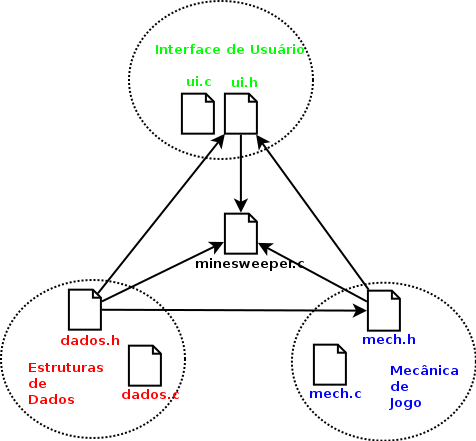
\includegraphics[width=0.5\textwidth]{diagrama.png}
\caption{Módulos e Arquivos do Projeto}
\end{figure}

\subsection{Estruturas de Dados}
Neste módulo são implementadas estruturas de dados auxiliares, como vetores para coordenadas em 2-D, e estruturas de dados básicas do jogo, como o tabuleiro do campo minado, e suas interfaces de programação, tal como métodos para criação e destruição destas, e métodos para manipulação de seus estados internos e dados armazenados.

\subsubsection{Estrutura ``vec''}
Esta estrutura é uma simples estrutura para armazenamento de coordenadas cartesianas 2-D inteiras no primeiro quadrante. Não possui métodos implementados.

\begin{tabular}{| c | c | l |}
\hline Nome da estrutura & \multicolumn{2}{c |}{vec}\\
\hline Nome do Campo & Tipo & Descrição\\
\hline x & \textbf{unsigned} & Componente cartesiana em $x$\\
y & \textbf{unsigned} & Componente cartesiana em $y$\\
\hline
\end{tabular}

\subsubsection{Estrutura ``jogada\_t''}
Esta estrutura tem a função de servir como estrutura de dados auxiliar, transportando o código e coordenada de uma jogada realizada pelo usuário. Possui métodos {\it getters} e {\it setters}.\\\\
\begin{tabular}{| c | c | l |}
\hline Nome da estrutura & \multicolumn{2}{c |}{jogada\_t}\\
\hline Nome do Campo & Tipo & Descrição\\
\hline v & \textbf{vec} & Coordenada cartesiana do ponto da jogada\\
opjogada & \textbf{char} & Código da jogada\\
\hline
\end{tabular}

\paragraph{Métodos}
\begin{itemize}
\item \textbf{char} {\it get\_jogada}(\textbf{jogada\_t} tab) : Retorna o código da jogada armazenada em uma estrutura \textbf{jogada\_t}.
\item \textbf{void} {\it set\_jogada}(\textbf{jogada\_t*} tab, \textbf{char} op) : Armazena um código de jogada em uma estrutura \textbf{jogada\_t}.
\item \textbf{vec} {\it get\_coord}(\textbf{jogada\_t} jogada) : Retorna a coordenada armazenada em uma estrutura \textbf{jogada\_t}.
\item \textbf{void} {\it set\_coord}(\textbf{jogada\_t*} jogada, \textbf{unsigned} x, \textbf{unsigned} y) : Armazena uma coordenada em uma estrutura \textbf{jogada\_t}.
\end{itemize}

\subsubsection{Estrutura ``tabuleiro\_t''}
Nesta estrutura são armazenadas informações sobre o tabuleiro do campo minado, tais como suas dimensões, número de minas semeadas, e dois vetores armazenando o estado atual do tabuleiro, uma máscara das casas livres, e informações sobre as minas e dicas de suas localizações. Possui métodos para inicialização, destruição, {\it getters} e {\it setters}.\\\\
\begin{tabular}{| c | c | l |}
\hline Nome da estrutura & \multicolumn{2}{c |}{tabuleiro\_t}\\
\hline Nome do Campo & Tipo & Descrição\\
\hline m & \textbf{unsigned} & Número de linhas do tabuleiro \\
n & \textbf{unsigned} & Número de colunas do tabuleiro\\
q & \textbf{unsigned} & Número de minas semeadas\\
usr & \textbf{char*} & Vetor máscara do tabuleiro\\
gabarito & \textbf{char*} & Vetor das minas e dicas do tabuleiro \\
\hline
\end{tabular}

\paragraph{Métodos}
\subparagraph{Inicialização e Destruição}
\begin{itemize}
\item \textbf{void} {\it inicializa\_tab}(\textbf{tabuleiro\_t*} tab) : Aloca espaço para os vetores da estrutura \textbf{tabuleiro\_t} de acordo com as dimensões armazenadas.
\item \textbf{void} {\it destroi\_tab}(\textbf{tabuleiro\_t*} tab) : Libera o espaço alocado para os vetores da estrutura \textbf{tabuleiro\_t}.
\end{itemize}
\subparagraph{\textit{Getters}}
\begin{itemize}
\item \textbf{unsigned} {\it get\_m}(\textbf{tabuleiro\_t} tab) : Retorna a dimensão vertical do tabuleiro.
\item \textbf{unsigned} {\it get\_n}(\textbf{tabuleiro\_t} tab) : Retorna a dimensão horizontal do tabuleiro.
\item \textbf{unsigned} {\it get\_q}(\textbf{tabuleiro\_t} tab) : Retorna o número de minas do tabuleiro.
\item \textbf{char} {\it get\_usr}(\textbf{tabuleiro\_t} tab, \textbf{vec} v) : Retorna o conteúdo de uma determinada coordenada \textbf{v} do tabuleiro máscara.
\item \textbf{char} {\it get\_gabarito}(\textbf{tabuleiro\_t} tab, \textbf{vec} v) : Retorna o conteúdo de uma determinada coordenada \textbf{v} do tabuleiro das minas e dicas.
\end{itemize}
\subparagraph{\textit{Setters}}
\begin{itemize}
\item \textbf{void} {\it set\_m}(\textbf{tabuleiro\_t*} tab, \textbf{unsigned} m) : Armazena a dimensão vertical do tabuleiro.
\item \textbf{void} {\it set\_n}(\textbf{tabuleiro\_t*} tab, \textbf{unsigned} n) : Armazena a dimensão horizontal do tabuleiro.
\item \textbf{void} {\it set\_q}(\textbf{tabuleiro\_t*} tab, \textbf{unsigned} q) : Armazena o número de minas do tabuleiro.
\item \textbf{void} {\it set\_usr}(\textbf{tabuleiro\_t*} tab, \textbf{vec} v, \textbf{char} usr) : Armazena um caractere \textbf{usr} em uma determinada coordenada \textbf{v} do tabuleiro máscara.
\item \textbf{void} {\it set\_gabarito}(\textbf{tabuleiro\_t*} tab, \textbf{vec} v, \textbf{char} gabarito) : Armazena um caractere \textbf{gabarito} em uma determinada coordenada \textbf{v} do tabuleiro das minas e dicas.
\end{itemize}
\subsection{Mecânica de Jogo}
Neste módulo são implementadas funções relacionadas ao funcionamento do jogo, tal como rotinas para processar condições de vitória, ou rotinas para determinar os resultados de uma jogada efetuada pelo usuário. Não possui estruturas próprias. Depende do módulo \textbf{Estruturas de Dados}.
\subsubsection{Função CriarTabuleiroUsr}
\paragraph{Sintaxe}
\textbf{void} {\it CriarTabuleiroUsr}(\textbf{tabuleiro\_t*} usr);\\
Preenche o tabuleiro máscara da estrutura \textbf{tabuleiro\_t} apontado por \textbf{usr} com asteriscos, colocando-no no estado inicial.
\subsubsection{Função ColocarBombas}
\paragraph{Sintaxe}
\textbf{void} {\it ColocarBombas}(\textbf{tabuleiro\_t*} gabarito);\\
Semeia o número de bombas configurado na estrutura \textbf{tabuleiro\_t} apontada por \textbf{gabarito}.
\subsubsection{Função AvaliarVizinhos}
\paragraph{Sintaxe}
\textbf{void} {\it AvaliarVizinhos}(\textbf{tabuleiro\_t*} gabarito);\\
Preenche o tabuleiro máscara da estrutura \textbf{tabuleiro\_t} apontado por \textbf{gabarito} com dicas da presença de bombas na vizinhança de cada casa.
\subsubsection{Função Revela}
\paragraph{Sintaxe}
\textbf{void} {\it Revela}(\textbf{tabuleiro\_t*} gabarito, \textbf{vec} v);\\
Dada uma coordenada \textbf{v}, e uma estrutura \textbf{tabuleiro\_t} apontado por gabarito, revela as casas vizinhas à \textbf{v} no tabuleiro máscara da estrutura, tendo como fronteira, casas contendo dicas diferentes de zero.
\subsubsection{Função ExecutaJogada}
\paragraph{Sintaxe}
\textbf{void} {\it ExecutaJogada}(\textbf{tabuleiro\_t*} gabarito, \textbf{jogada\_t*} jogada, \textbf{int*} p);\\
Verifica o resultado de uma jogada, sendo \textbf{gabarito} um ponteiro para uma estrutura \textbf{tabuleiro\_t}, \textbf{jogada} um ponteiro para a estrutura \textbf{jogada\_t} da jogada a ser realizada, e \textbf{p} um ponteiro para a variável contador do número de minas marcadas corretamente.
\subsubsection{Função ConfereRevelados}
\paragraph{Sintaxe}
\textbf{int} {\it ConfereRevelados}(\textbf{tabuleiro\_t} tab);\\
Testa se o tabuleiro máscara da estrutura \textbf{tabuleiro\_t} apontada por \textbf{tab} já foi completamente revelado. Retorna 1 se \textbf{tab} foi completamente revelado, 0 no caso contrário.
\subsection{Interface de Usuário}
Neste módulo são implementadas funções relacionadas à interface do usuário com o jogo. Nisto inclui-se por exemplo a exibição do tabuleiro em seu estado atual na tela, ou a captura dos comandos e jogadas do usuário. Depende do módulo \textbf{Estruturas de Dados}.
\subsubsection{Função menu}
\paragraph{Sintaxe}
\textbf{int} {\it menu}();\\
Imprime uma mensagem de início do jogo seguida de um menu de opções. Retorna o número da opção digitada.
\subsubsection{Função opseguir}
\paragraph{Sintaxe}
\textbf{void} {\it opseguir}(\textbf{tabuleiro\_t*} p, \textbf{int*} i);\\
Chama a função \textbf{menu()}, trata a opção retornada e captura dimensões para um novo tabuleiro. \textbf{p} é ponteiro para a estrutura \textbf{tabuleiro\_t} a ser configurada, e \textbf{i} é ponteiro para uma \textbf{int} onde será armazenada a opção escolhida(1 se o jogo deve começar e 0 se deve sair do jogo).
\subsubsection{Função fimDeJogo}
\paragraph{Sintaxe}
\textbf{void} {\it fimDeJogo}(\textbf{int} i, \textbf{tabuleiro\_t} tab);\\
Imprime uma mensagem de fim de jogo adequada à condição de término da partida. \textbf{i} é o número de minas descobertas, \textbf{tab} é o tabuleiro da partida.
\subsubsection{Função lerJogada}
\paragraph{Sintaxe}
\textbf{void} {\it lerJogada}(\textbf{jogada\_t*} jog, \textbf{tabuleiro\_t} tab);\\
Captura uma jogada digitada pelo usuário. \textbf{jog} é o ponteiro para a estrutura \textbf{jogada\_t} onde deve ser armazenada a jogada, \textbf{tab} é o tabuleiro da partida.
\subsubsection{Função imprimirTabuleiro}
\paragraph{Sintaxe}
\textbf{void} {\it imprimirTabuleiro}(\textbf{tabuleiro\_t} tab);\\
Imprime o tabuleiro \textbf{tab} formatado na tela.
\section{Ferramentas}
Visando simplificar e eliminar algumas dificuldades do processo de desenvolvimento, escolhemos fazer uso de algumas ferramentas em software.
\subsection{Git}
O \textbf{Git} é um sistema de controle de versão distribuído. Este sistema permite que a equipe simplesmente clone os arquivos do projeto armazenado em um repositório on-line, trabalhe em simultâneo, localmente e independentemente, em suas cópias, fazendo todas as modificações necessárias, enviando ao fim suas alterações ao repositório sem grandes problemas no momento de integrar as modificações. Isto se deve a uma das facilidades do sistema de versionamento, que trata automaticamente quase todos os conflitos causados pelas modificações, além da facilidade adicionada de todos os integrantes sempre poderem receber o projeto em sua forma mais atual sem necessitarem cloná-lo por completo novamente. Com o \textbf{Git} ainda há a possibilidade de reverter modificações específicas ou ainda de desenvolver uma versão alternativa do projeto em paralelo com a original, sem afetar o andamento do restante do projeto.

O repositório do projeto pode ser encontrado em \url{https://github.com/K17K47/minesweeper}

\subsection{make}
Reconhecendo o número de arquivos presentes no projeto, realizar uma compilação manualmente se torna uma operação laboriosa, e passível de erros que afetam o desempenho do processo de teste e desenvolvimento. Assim optamos por usar o \textbf{GNU make}, uma versão de uma ferramenta de automação de compilação, que por meio de um pequeno script, que para projetos simples como o atual não precisa ser reescrito, mesmo com intensas modificações, é capaz de reduzir o ato de compilação, neste projeto, de 5 comandos no terminal para apenas 1. Para compilar, estando na pasta ``src'' do repositório, basta executar ``make''.

\subsection{\LaTeX}
Visando facilitar também a escrita da documentação e do relatório do projeto, optamos por escrevê-lo em \LaTeX, um sistema de diagramação de textos, amplamente utilizado na escrita de documentos oficiais, artigos científicos e livros devido à sua alta qualidade tipográfica. Este sistema reduz a escrita de um texto formatado à escrita de um arquivo em uma linguagem de descrição de alto nível, desacoplando a aparência do texto de seu conteúdo, e permitindo sua compilação em diversas plataformas, mantendo ainda a mesma aparência. Este documento foi escrito com o \LaTeXe.

\chapter{Conclusão}
Vimos durante o andamento do projeto que, por mais simples que o mesmo seja, sempre há dificuldades a serem vencidas, e que estas existem nas mais diversas formas: de um código mal-formatado escondendo erros, até alterações causando regressões. Mas que sobre tudo, sempre existem práticas e ferramentas, que se não as resolvem, amenizam e simplificam o processo.

Concluimos também que o trabalho em equipe apesar de reduzir a carga de cada integrante, requer cuidadosa organização para que seja eficiente. Ao fim, foi uma atividade bastante educativa, e por isso, constitui uma ótima experiência para todos no grupo.
\end{document}